\documentclass[12pt]{article}
\usepackage{a4wide}
\usepackage{graphicx}
\usepackage{color, amssymb}
\usepackage[english,greek]{babel}
\usepackage[utf8]{inputenc}
\usepackage{color} 
\usepackage{geometry} %Για να προσαρμώσω το  margin της σελλίδας.
\usepackage{fancyvrb} 
\usepackage{ragged2e} %Για πλήρης στίχηση.
\usepackage{listings} %Για να μπορώ να βάζω κώδικα.
\usepackage{array}
\renewcommand{\baselinestretch}{1.1}
\input{epsf}

\setlength{\parindent}{1em}

\geometry{left = 1in, right = 1in, top= 1in, bottom = 1in}


\lstdefinestyle{mystyle}{       %Ορισμός του style του κώδικα.
    language=Matlab,
    % Adjust the appearance as needed:
    basicstyle=\small\ttfamily,
    numbers=left,
    numberstyle=\tiny,
    numbersep=5pt,
    frame=single,
    breaklines=true,
    breakatwhitespace=true,
    tabsize=2,
    captionpos=b,
}
\lstset{style=mystyle}


\begin{document}


\noindent\rule{\textwidth}{2pt}
\begin{center}
\vskip -.5 cm

{\bf ΠΟΛΥΤΕΧΝΕΙΟ ΚΡΗΤΗΣ}\\
{\bf ΣΧΟΛΗ ΗΜΜΥ}\\
{\bf Τηλεπικοινωνιακά Συστήματα Ι} \\
Παράδωση 2ης εργασίας \\
Ημερομηνία Παράδοσης: 25/05/2024

\end{center}
\vskip -.8cm
\rule{\textwidth}{.5pt}

\vskip .2cm
\noindent
\begin{center}
	\vspace{2cm}
	{\LARGE Ομάδα 120 }\\	
	\vspace{2cm}
\begin{tabular}{|p{4cm}|p{4cm}|p{4cm}|}
	\hline
Επώνυμο &  Δήμας & Λαμπράκης\\
    \hline 
Όνομα & Χρήστος  & Μιχάλης   \\
\hline 
Α.Μ. & 2021030183  & 2020030077 \\
\hline 
	
\end{tabular}
\end{center}

\vspace{2cm}

\begin{center}
	Πλήθος ωρών ενασχόλησης:{\bf 15}
\end{center}

\newpage


%%%%%%%%%%%%%%%%%  Θ1
\begin{justify}
{\bf  Θ.1} (10) Για κάθε $T>0$ υπολογίστε το ολοκλήρωμα και σχεδιάστε
την συνάρτηση αυτοομοιότητας της συνάρτησης:
\end{justify}

\[
    \phi(t) =
\left\{
	\begin{array}{ll}
		\frac{1}{\sqrt{T}} &, \mbox{αν } |t| \leq \frac{T}{2} \\
		0 &, \mbox{διαφορετικά.}
	\end{array}
\right.
\]


\begin{justify}
\textbf{Λύση:}\\
H συνάρτηση αυτοομοιότητας της $\phi(t)$ ορίζεται ως $R_{\phi\phi}(\tau)=\int_{-\infty}^{+\infty} \phi(t+\tau)\phi(t)\,d\tau, \hspace{1.5em} \forall t \epsilon \mathbb{R}$.\\
Επιπλέον το $\phi(t+\tau)$:
    
\[
    \phi(t+\tau) =
\left\{
	\begin{array}{ll}
		\frac{1}{\sqrt{T}} &, \mbox{αν } |t+\tau| \leq \frac{T}{2} \\
		0 &, \mbox{διαφορετικά.}
	\end{array}
\right.
\]
\end{justify}

\begin{justify}
    
Παρατηρούμε ότι:
\newline
$\int_{-\infty}^{+\infty} \phi(t+\tau)\phi(t)\,d\tau, 
                                        \hspace{1.5em} t=s-\tau$
\newline
$\int_{-\infty}^{+\infty} \phi(s)\phi(s-\tau)\,ds, 
                                        \hspace{1.5em} s=\tau-u$
\newline
$\int_{-\infty}^{+\infty} \phi(\tau-u)\phi(-u)\,du, 
                                        \hspace{1.5em} \phi(-u)=g(u)$
                                        \newline
$\int_{-\infty}^{+\infty} \phi(\tau-u)g(u)\,du = \phi(\tau)*g(\tau)=\phi(\tau)*\phi(-\tau)$
\end{justify}

%%%%%%%%%Περιπτωση Θ1.1
\begin{justify}
Άρα με βάση την μεθοδολογία της συνέλιξης καταλήγουμε στις εξής περιπτώσεις:\newline\newline
{\bf 1\textsuperscript{η} Περίπτωση:}  $\tau+T<-\frac{T}{2}$
\[
R_{\phi\phi}(\tau)=0, \forall \tau \epsilon (-\infty,-T)      
\]
\end{justify}

%%%%%%%%%Περιπτωση Θ1.2
\begin{justify}
{\bf 2\textsuperscript{η} Περίπτωση:}  $\tau+\frac{T}{2}\geq -\frac{T}{2}$ και 
$\tau-\frac{T}{2}< -\frac{T}{2}$ 
\[
R_{\phi\phi}(\tau)=\int_{-\frac{T}{2}}^{\tau+\frac{T}{2}} \phi(t+\tau)\phi(t)\,d\tau =
\int_{-\frac{T}{2}}^{\tau+\frac{T}{2}} \frac{1}{\sqrt{T}}\frac{1}{\sqrt{T}}\,d\tau =
\frac{1}{T}[\tau]_{-\frac{T}{2}}^{\tau+\frac{T}{2}}
= \frac{1}{T}(\tau+\frac{T}{2}+\frac{T}{2})=1+\frac{\tau}{T} \hspace{1.5em} \forall\tau\epsilon[-T,0)\]
\end{justify}

%%%%%%%%%Περιπτωση Θ1.3
\begin{justify}
{\bf 3\textsuperscript{η} Περίπτωση:} $\tau-\frac{T}{2}\geq -\frac{T}{2}$ και 
$\tau-\frac{T}{2}< \frac{T}{2}$ 
\[
R_{\phi\phi}(\tau)=\int_{\tau-\frac{T}{2}}^{\frac{T}{2}} \frac{1}{T}\,d\tau = 
\frac{1}{T}[\tau]_{\tau-\frac{T}{2}}^{\frac{T}{2}} = \frac{1}{T}(\frac{T}{2}-\tau+\frac{T}{2})
=1-\frac{\tau}{T} \hspace{1.5em} \forall\tau\epsilon[0,T)
\]
\end{justify}

%%%%%%%%%Περιπτωση Θ1.4
\begin{justify}
{\bf 4\textsuperscript{η} Περίπτωση:}  $\tau-\frac{T}{2}\geq\frac{T}{2}$
\[
R_{\phi\phi}(\tau)=0, \forall \tau \epsilon [T,+\infty)      
\]
\end{justify}

\newpage

\begin{justify}
Οπότε:
\[
R_{\phi\phi}(\tau)= 
\left\{
	\begin{array}{lll}
		1+\frac{\tau}{T} &, \mbox{αν } -T \leq \tau < 0 \\
        1-\frac{\tau}{T} &, \mbox{αν } 0 \leq \tau < T \\
		0 &, \mbox{διαφορετικά.}
	\end{array}
\right.
\]
\end{justify}

%%%%%%PLOT
\begin{center}
    \centering
    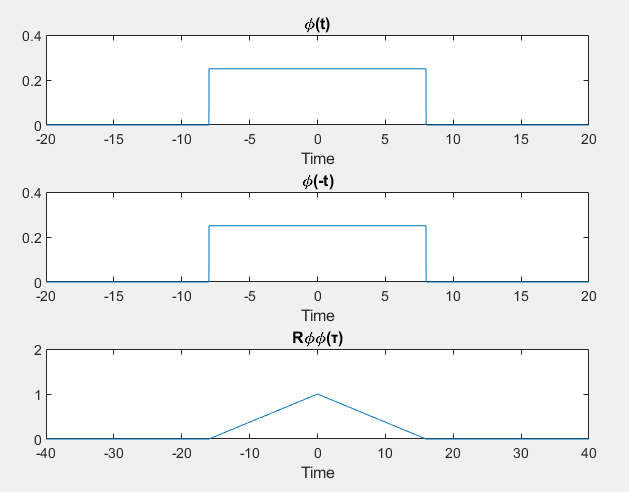
\includegraphics[width=0.8\textwidth]{THETA/Images/theta.fig1.png} % Adjust width as neededfilename of your images
    \label{fig:third_image}
\end{center}


%%%%%%%%%%%%%%%%%  Θ2
\begin{justify}
{\bf  Θ.2} (10) Επαναλάβετε την ίδια διαδικασία για $\phi(t-2)$.\\\\
\textbf{Λύση:}\\
Αρχικά θα υπολογίσουμε την $\phi(t-2)$:
\[
    \phi(t-2) =
\left\{
	\begin{array}{ll}
		\frac{1}{\sqrt{T}} &, \mbox{αν} -\frac{T}{2}+2 \leq t \leq \frac{T}{2} + 2 \\
		0 &, \mbox{διαφορετικά.}
	\end{array}
\right.
\]
\end{justify}

\begin{justify}
H συνάρτηση αυτοομοιότητας της $\phi(t)$ ορίζεται ως $R_{\phi\phi}=\int_{-\infty}^{+\infty} \phi(t-2+\tau)\phi(t-2)\,d\tau, \hspace{1.5em} \forall t \epsilon \mathbb{R}$.\newline
Βάση του {\bf Θ.1} προχωράμε στη συνέλιξη και καταλήγουμε στις εξής περιπτώσεις:
\end{justify}

%%%%%%%%%Περιπτωση Θ2.1
\begin{justify}
{\bf 1\textsuperscript{η} Περίπτωση:}  $\tau+\frac{T}{2}+2<-\frac{T}{2}$
\[
R_{\phi\phi}(\tau)=0, \forall \tau \epsilon (-\infty,-T)      
\]
\end{justify}

%%%%%%%%%Περιπτωση Θ2.2
\begin{justify}
{\bf 2\textsuperscript{η} Περίπτωση:}  $\tau+\frac{T}{2}+2\geq-\frac{T}{2}$ και $\tau-\frac{T}{2}+2<-\frac{T}{2} $
\[
R_{\phi\phi}(\tau)=\int_{-\frac{T}{2}+2}^{\tau+2+\frac{T}{2}} \frac{1}{T}\,d\tau = 
\frac{1}{T}[\tau]_{-\frac{T}{2}+2}^{\tau+2+\frac{T}{2}} = \frac{\tau+2+\frac{T}{2}+\frac{T}{2}-2}{T}
=1+\frac{\tau}{T} \hspace{1.5em} \forall\tau\epsilon[-T,0)
\]
\end{justify}

%%%%%%%%%Περιπτωση Θ2.3
\begin{justify}
{\bf 3\textsuperscript{η} Περίπτωση:}  $\tau-\frac{T}{2}+2\geq-\frac{T}{2}$ και $\tau-\frac{T}{2}+2<\frac{T}{2} $
\[
R_{\phi\phi}(\tau)=\int_{\tau-\frac{T}{2}+2}^{\frac{T}{2}+2} \frac{1}{T}\,d\tau = 
\frac{1}{T}[\tau]_{\tau-\frac{T}{2}+2}^{\frac{T}{2}+2} = \frac{\frac{T}{2}-\tau+\frac{T}{2}}{T}
=1-\frac{\tau}{T} \hspace{1.5em} \forall\tau\epsilon[0,T)
\]
\end{justify}

%%%%%%%%%Περιπτωση Θ2.4
\begin{justify}
{\bf 4\textsuperscript{η} Περίπτωση:}  $\tau-\frac{T}{2}+2\geq\frac{T}{2}$
\[
R_{\phi\phi}(\tau)=0, \forall \tau \epsilon [T,+\infty)      
\]
\end{justify}

\vspace{0.5cm}

\begin{justify}
Οπότε τελικά:
\[
R_{\phi\phi}(\tau)= 
\left\{
	\begin{array}{lll}
		1+\frac{\tau}{T} &, \mbox{αν } -T \leq \tau < 0 \\
        1-\frac{\tau}{T} &, \mbox{αν } 0 \leq \tau < T \\
		0 &, \mbox{διαφορετικά.}
	\end{array}
\right.
\]
\end{justify}

%%%%%%PLOT
\begin{center}
    \centering
    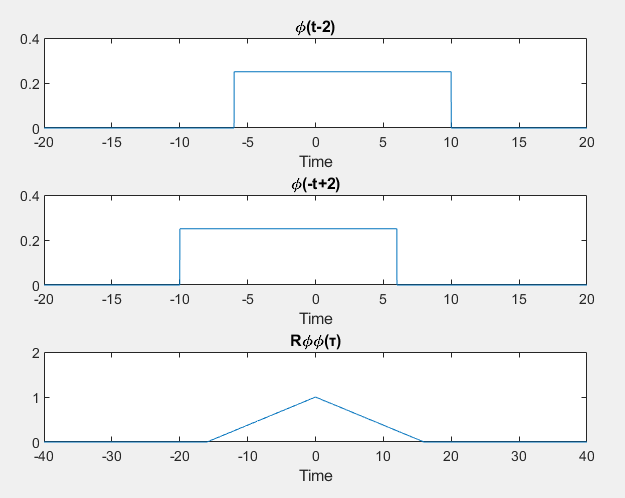
\includegraphics[width=0.8\textwidth]{THETA/Images/theta.fig2.png} % Adjust width as neededfilename of your images
    \label{fig:third_image}
\end{center}


\begin{justify}
Παρατηρούμε ότι οι συναρτήσεις αυτοομοιότητας των ερωτημάτων {\bf Θ.1} και {\bf Θ.2} είναι πανομοιότυπες. Λόγω αυτού βγαίνει το συμπέρασμα πως η $R_{\phi\phi}(\tau)$ δεν επηρεάζεται από τις χρονικές μετατοπίσεις της $\phi(t)$.
\end{justify}

\newpage


%%%%%%%%%%%%%%%%%  Θ3
\begin{justify}
{\bf  Θ.3} (10)Να επαναλάβετε για την:
\[
\phi(t)= 
\left\{
	\begin{array}{lll}
		\frac{1}{\sqrt{T}} &, \mbox{αν } 0 \leq t < \frac{T}{2} \\
        -\frac{1}{\sqrt{T}} &, \mbox{αν } \frac{T}{2} \leq t \leq T \\
		0 &, \mbox{διαφορετικά.}
	\end{array}
\right.
\]
\end{justify}

\begin{justify}
\textbf{Λύση:}\\
Θα κινηθούμε όμοια με το {\bf Θ.1} οπότε:
\[
\phi(t+\tau)= 
\left\{
	\begin{array}{lll}
		\frac{1}{\sqrt{T}} &, \mbox{αν } 0 \leq t+\tau < \frac{T}{2} \\
        -\frac{1}{\sqrt{T}} &, \mbox{αν } \frac{T}{2} \leq t+\tau \leq T \\
		0 &, \mbox{διαφορετικά.}
	\end{array}
\right.
\]
και καταλήγουμε στις εξής περιπτώσεις της συνέλιξης:
\end{justify}

%%%%%%%%%Περιπτωση Θ3.1
\begin{justify}
{\bf 1\textsuperscript{η} Περίπτωση:}  $\tau+T<0$
\[
R_{\phi\phi}(\tau)=0, \forall \tau \epsilon (-\infty,-T)      
\]
\end{justify}

%%%%%%%%%Περιπτωση Θ3.2
\begin{justify}
{\bf 2\textsuperscript{η} Περίπτωση:}  $\tau+T\geq0$ και $\tau+\frac{T}{2}<0$
\[
R_{\phi\phi}(\tau)=\int_{0}^{\tau+T} -\frac{1}{\sqrt{T}}\frac{1}{\sqrt{T}}\,d\tau =
\int_{0}^{\tau+T} -\frac{1}{T}\,d\tau=
-\frac{1}{T}[\tau]_{0}^{\tau+T} =\frac{-\tau-T}{T}
=-1-\frac{\tau}{T} \hspace{1.5em} \forall\tau\epsilon[-T,-\frac{T}{2})
\]
\end{justify}

%%%%%%%%%Περιπτωση Θ3.3
\begin{justify}
{\bf 3\textsuperscript{η} Περίπτωση:}  $\tau+\frac{T}{2}\geq0$ και $\tau<0$
\[
R_{\phi\phi}(\tau)=\int_{0}^{\tau+\frac{T}{2}}\frac{1}{T}\,d\tau+
\int_{\tau+\frac{T}{2}}^{\frac{T}{2}}-\frac{1}{T}\,d\tau+
\int_{\frac{T}{2}}^{\tau+T}\frac{1}{T}\,d\tau
=\frac{1}{T}([\tau]_{0}^{\tau+\frac{T}{2}}-[\tau]_{\tau+\frac{T}{2}}^{\frac{T}{2}}+
[\tau]_{\frac{T}{2}}^{\tau+T})
\]
\[
=\frac{1}{T}(\tau+\frac{T}{2}-\frac{T}{2}+\tau+\frac{T}{2}+\tau+T-\frac{T}{2})
=1+\frac{3\tau}{T}\hspace{1.5em} \forall\tau\epsilon[-\frac{T}{2},0)
\]
\end{justify}

%%%%%%%%%Περιπτωση Θ3.4
\begin{justify}
{\bf 4\textsuperscript{η} Περίπτωση:}  $\tau\geq0$ και $\tau<\frac{T}{2}$
\[
R_{\phi\phi}(\tau)=\int_{\tau}^{\frac{T}{2}}\frac{1}{T}\,d\tau+
\int_{\frac{T}{2}}^{\tau+\frac{T}{2}}-\frac{1}{T}\,d\tau+
\int_{\tau+\frac{T}{2}}^{T}\frac{1}{T}\,d\tau
=\frac{1}{T}([\tau]_{\tau}^{\frac{T}{2}}-[\tau]_{\frac{T}{2}}^{\tau+\frac{T}{2}}+
[\tau]_{\tau+\frac{T}{2}}^{T})
\]
\[
=\frac{1}{T}(\frac{T}{2}-\tau-\tau-\frac{T}{2}+\frac{T}{2}+T-\tau-\frac{T}{2})
=1-\frac{3\tau}{T}\hspace{1.5em} \forall\tau\epsilon[0,\frac{T}{2})
\]
\end{justify}

\newpage

%%%%%%%%%Περιπτωση Θ3.5
\begin{justify}
{\bf 5\textsuperscript{η} Περίπτωση:}  $\tau\geq\frac{T}{2}$ και $\tau\leq T$
\[
R_{\phi\phi}(\tau)=\int_{\tau}^{T} -\frac{1}{T}\,d\tau=
-\frac{1}{T}[\tau]_{\tau}^{T} =\frac{\tau-T}{T}
=-1+\frac{\tau}{T} \hspace{1.5em} \forall\tau\epsilon[\frac{T}{2},T]
\]
\end{justify}

%%%%%%%%%Περιπτωση Θ3.6
\begin{justify}
{\bf 6\textsuperscript{η} Περίπτωση:}  $\tau>T$
\[
R_{\phi\phi}(\tau)=0, \forall \tau \epsilon (T,\infty)      
\]
\end{justify}

\begin{justify}
Οπότε τελικά:
\[
R_{\phi\phi}(\tau)= 
\left\{
	\begin{array}{lllll}
		-1-\frac{\tau}{T} &, \mbox{αν } -T \leq \tau < -\frac{T}{2} \\
        1+\frac{3\tau}{T} &, \mbox{αν }  -\frac{T}{2} \leq \tau <0\\
        1-\frac{3\tau}{T} &, \mbox{αν } 0 \leq \tau <\frac{T}{2}\\
        -1+\frac{\tau}{T} &, \mbox{αν } \frac{T}{2} \leq \tau \leq T\\
		0 &, \mbox{διαφορετικά.}
	\end{array}
\right.
\]
\end{justify}

\vspace{1cm}

%%%%%%PLOT
\begin{center}
    \centering
    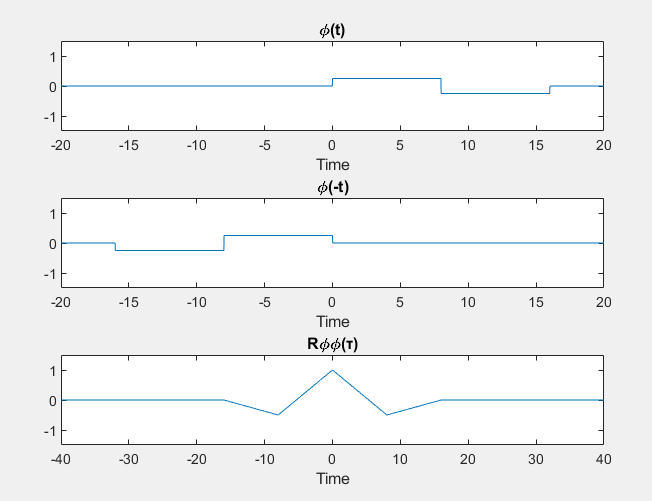
\includegraphics[width=0.8\textwidth]{THETA/Images/theta.fig3.png} % Adjust width as neededfilename of your images
    \label{fig:third_image}
\end{center}


\newpage

%%%%%%%%%%%%%%%%%  A1

\begin{justify}
    {\bf  Α.1} Να δημιουργήσετε παλμό \textlatin{SRRC} $\phi(t)$
    με τιμές  $T = 10^{-3} sec$, $over=10$, 
    $T\textsubscript{\textlatin{s}}=\frac{T}{over}$, $A=4$, και 
    $\alpha = 0.5$.
\end{justify}

\begin{justify}
    (10) Μέσω των συναρτήσεων \textlatin{fftshift} και
    \textlatin{fft}, να υπολογίσετε το μέτρο του μετασχηματισμού
    \textlatin{Fourier} της $\phi(t)$, $|\Phi(F)|$, 
    σε $N\textsubscript{\latintext{f}}$ ισαπέχοντα σημεία στο διάστημα
    $[-\frac{F\textsubscript{\textlatin{s}}}{2},\frac{F\textsubscript{\textlatin{s}}}{2}]$.
    Να σχεδιάσετε τη φασματική πυκνότητα ενέργειας $|\Phi(F)|^{2}$
    στον κατάληλλο άξονα συχνοτήτων με χρήσης της εντολής \textlatin{semiilogy}.
\end{justify}

\begin{justify}
    {\bf Λύση:}\\\\
    Έγινε χρήση της συνάρτησης $srrc\_pulse.m$ και
    επιλέγοντας τιμή $N_f=4096$ (για να μην υπάρξουν
    παραμορφώσεις).
\end{justify}

%%%%%%PLOT
\begin{center}
    \centering
    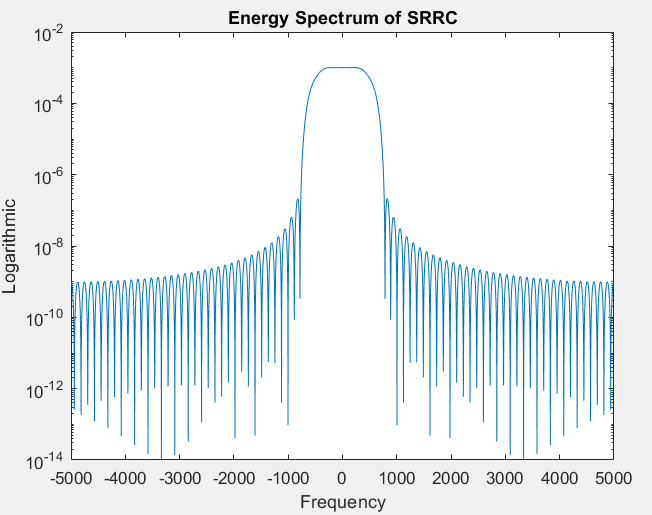
\includegraphics[width=0.8\textwidth]{ALPHA/images/a1.png} % Adjust width as neededfilename of your images
\end{center}


\begin{justify}
    και ο κώδικας \textlatin{Matlab}:
\end{justify}

\vspace{-1cm}

%%%%%%%%MATLAB code
\textlatin{
    \lstinputlisting[language=Matlab,]{ALPHA/Matlab/a1.1.m}
} 

\newpage

%%%%%%%%%%%%%%%%%  A2

\begin{justify}
    {\bf Α.2} Να δημιουργήσετε ακολουθία $N=100$ ανεξάρτητων και
    ισοπίθανων $bits \{b\textsubscript{0},...,b\textsubscript{Ν-1}\}$.
    Χρησιμοποιώντας την απεικόνιση
    \[ 0 \rightarrow +1, \]
    \[ 1 \rightarrow -1, \]
    να απεικονίσετε τα \textlatin{bits} σε σύμβολα 
    Χ\textsuperscript{\textlatin{n}} για  $n=0,...,N-1$.\\
    Να κατασκευάσετε την κυματομορφή:
    \[
        X(t) = \sum_{n=0}^{N-1} X\textsubscript{\textlatin{n}}\phi(t-nT).   
    \]
\end{justify}

\begin{justify}
    {\bf Λύση:}\\\\
    Αρχικά δημιουργήθηκε η ακολουθία \textlatin{bits} 
    και έπειτα μέσω της συνάρτησης $bits\_to\_2PAM$
    μετατράπηκαν σε \textlatin{2-PAM} σύμβολα. 
\end{justify}

%%%%%%PLOT
\begin{center}
    \centering
    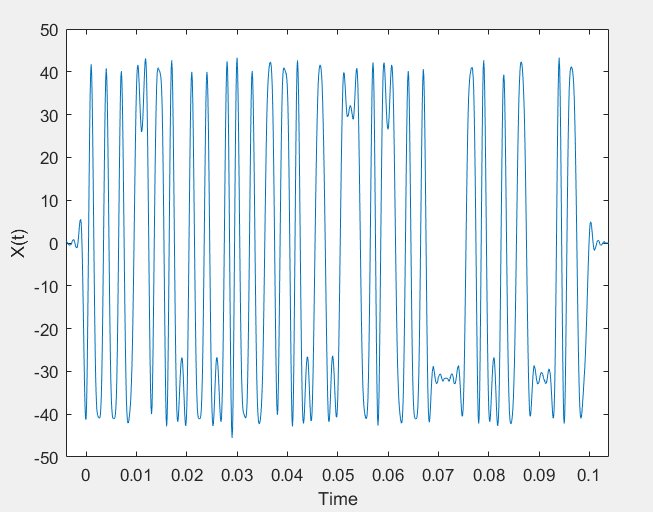
\includegraphics[width=0.8\textwidth]{ALPHA/images/a2.png} % Adjust width as neededfilename of your images
\end{center}

\newpage

\begin{justify}
    και ο κώδικας \textlatin{Matlab}:
\end{justify}

\vspace{-0.8cm}

%%%%%%%%MATLAB code
\textlatin{
    \lstinputlisting[language=Matlab,]{ALPHA/Matlab/a2.m}
} 


\vspace*{2cm}


%%%%%%%%%%%%%%%%%  A3
\begin{justify}
    Υποθέτοντας ότι το πλήθος των συμβόλων είναι άπειρο, αποδείξαμε
    ότι η φασματική πυκνώτητα ισχύος του $X(t)$ είναι:
    \[
      S\textsubscript{Χ}{(F)} = \frac{\sigma^{2}\textsubscript{Χ}}{T}|\Phi(F)|^{2}.
    \]
    {\bf Α.3} (10) Με την χρήση των συναρτήσεων \textlatin{fft} και
    \textlatin{fftshift} να υπολογίσετε το περιοδόγραμμα μιάς 
    υλοποίησης της \textlatin{X(t)}:
    \[
        P\textsubscript{Χ}(F) = \frac{|F(X(t))|^{2}}{T\textsubscript{\textlatin{total}}}.  
    \]
    Να σχεδιάσετε το $P\textsubscript{Χ}(F)$ με χρήση 
    \textlatin{plot} και \textlatin{semilogy}.
\end{justify}

\newpage

\begin{justify}
    {\bf Λύση:}\\\\
    Παρακάτω παρουσιάζεται το περιοδόγραμμα $P_X(F)$
    σε δεκαδική και λογαριθμική κλίμακα:
\end{justify}

%%%%%%PLOT
\begin{center}
    \centering
    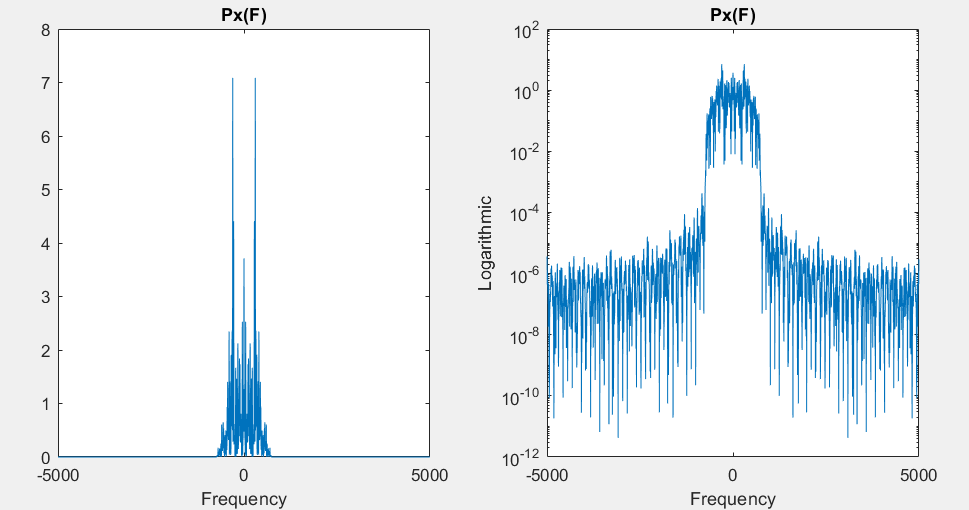
\includegraphics[width=0.8\textwidth]{ALPHA/images/a3.1.png} % Adjust width as neededfilename of your images
\end{center}


\begin{justify}
    και ο κώδικας \textlatin{Matlab}:
\end{justify}

\vspace{-0.8cm}

%%%%%%%%MATLAB code
\textlatin{
    \lstinputlisting[language=Matlab,]{ALPHA/Matlab/a2.m}
}

\newpage

\begin{justify}
    (10) Να εκτιμήσετε τη φασματική πυκνότητα ισχύος υπολογίζοντας
    αριθμιτικές μέσες τιμές πάνω σε K (ενδεικτικά, Κ=500) υλοποιήσεις
    περιοδογραμμάτων. Να σχεδιάσετε σε κοινό \textlatin{semilogy}
    την εκτίμηση και τη θεωριτική φασματική πυκνότητα ισχύος.
\end{justify}

\begin{justify}
    {\bf Λύση:}\\\\
    Έγιναν οι κατάληλλοι υπολογισμοί μέσω \textlatin{Matlab}
    και η εκτίμηση που πραγματοποιήθηκε συγκρίνεται με την
    θεωριτική φασματική πυκνότητα ισχύος η οποία προκύπτει
    από τον παραπάνω τύπο.\\\\
    Ο υπολογισμός της διασποράς $\sigma_X^2$ προκύπτει ως εξής:
    \[
        \sigma_X^2 = E[(X_n-E(X_n))^2]=E[X_n^2]=1
    \]
    Διότι: 
    \[
        E[X_n^2]=\sum x^2p_x=(1)^2\frac{1}{2}+(-1)^2\frac{1}{2}=1
    \]	
    Παρακάτω απεικονίζονται σε κοινό διάγραμμα ώστε να πραγματοποιηθεί
    η σύγκρισή τους: 
\end{justify}

%%%%%%PLOT
\begin{center}
    \centering
    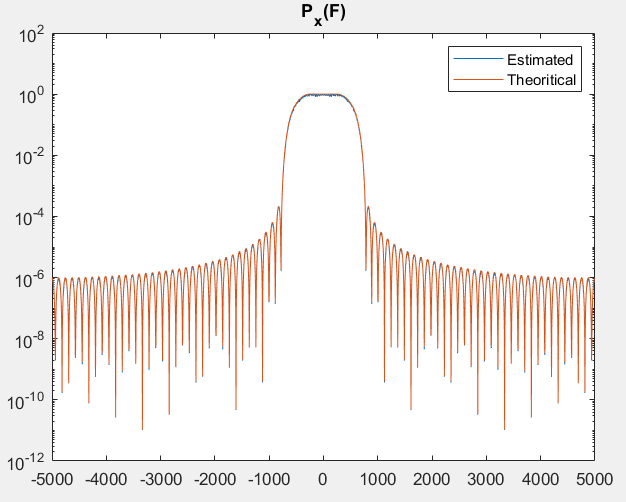
\includegraphics[width=0.8\textwidth]{ALPHA/images/a3.2.png} % Adjust width as neededfilename of your images
\end{center}

\newpage

\begin{justify}
    και ο κώδικας \textlatin{Matlab}:
\end{justify}


\vspace{-0.8cm}

%%%%%%%%MATLAB code
\textlatin{
    \lstinputlisting[language=Matlab,]{ALPHA/Matlab/a3.2.m}
}

\newpage

\begin{justify}
    (10) Όσο αυξάνετε το Κ και το Ν, θα πρέπει η προσέγγιση να γίνεται
    καλύτερη.Συμβαίνει αυτό στα πειράματά σας\textlatin{;} Μπορείτε να 
    εξηγήσετε αυτό το φαινόμενο\textlatin{;}
\end{justify}

\begin{justify}
    {\bf Λύση:}\\\\
    Παρατηρούμε ότι για Κ=500 που χρησιμοποιήθηκε παραπάνω
    η προσέγγιση είναι αρεκτά καλή καθώς οι διακυμάνσεις
    των δύο γραφικών παρουσιάζουν μεγάλη ομοιότητα.\\\\
    Χρησιμοποιώντας τον ίδιο κώδικα και αλλάζοντας τις τιμές
    των παραμέτρων Ν και Κ προκύπτουν τα παρακάτω διαγράμματα:
\end{justify}

%%%%%%PLOT
\begin{center}
    \centering
    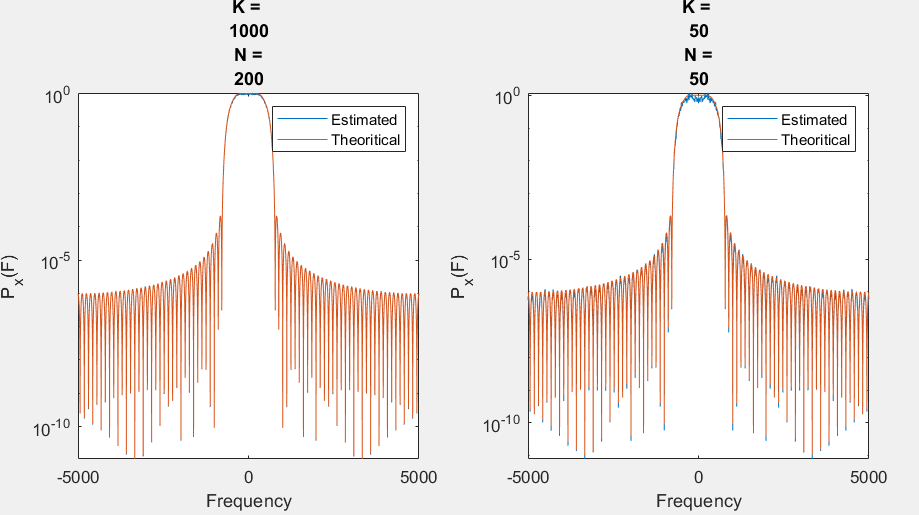
\includegraphics[width=0.8\textwidth]{ALPHA/images/a3.3.png} % Adjust width as neededfilename of your images
\end{center}

\begin{justify}
    και ο κώδικας \textlatin{Matlab}:
\end{justify}


\vspace{-0.8cm}

%%%%%%%%MATLAB code
\textlatin{
    \lstinputlisting[language=Matlab,]{ALPHA/Matlab/a3.3.m}
}


\begin{justify}
    Όπως επιβεβαιώνεται και από τα παραπάνω διαγράμματα, όσο
    αυξάνετε το Κ και το Ν, η προσέγγιση γίνεται καλύτερη.
    Αυτο συμβαίνει διότι τα περιοδογράμματα ακολουθούν κανονική
    κατανομή, όπως και τα \textlatin{bits} τα οποία
    κωδικοποιούνται και καταλήγουμε στην $X(t)$, οπότε
    όσο μεγαλύτερο γίνεται το δείγμα τόσο καλύτερη και πιο ακριβής
    γίνεται	η προσέγγιση.
\end{justify}

\newpage

%%%%%%%%%%%%%%%%%  A4

\begin{justify}
    {\bf A.4} Χρησιμοποιώντας την απεικόνιση:
    \[
      00 \rightarrow +3, 
    \]
    \[
      01 \rightarrow +1,
    \]
    \[
      11 \rightarrow -1,
    \]
    \[
      10 \rightarrow -3, 
    \]
    να κατασκευάσετε την ακολουθία 4-\textlatin{PAM} $X\textsubscript{\latintext{n}}$,
    για $n=0,...,\frac{N}{2}-1$.
\end{justify}

\begin{justify}
    {\bf Λύση:}\\\\
    Αρχικά κατασκευάστηκε η συνάρτηση $bits\_to\_4PAM$: 
\end{justify}

\vspace{-0.8cm}

%%%%%%%%MATLAB code
\textlatin{
    \lstinputlisting[language=Matlab,]{ALPHA/Matlab/bits_to4PAM.m}
}


\newpage

\begin{justify}
    Να κατασκευάσετε την κυματομορφή:
    \[
        X(t) = \sum_{n=0}^{\frac{N}{2}-1} X\textsubscript{\textlatin{n}}\phi(t-nT). 
    \]
    χρησιμοποιώντας την ίδια περίοδο $T$ με το ερώτημα {\bf Α.2}.
\end{justify}


\begin{justify}
    {\bf Λύση:}\\\\
    Όμοια με το ερώτημα {\bf Α.2}:
\end{justify}

%%%%%%PLOT
\begin{center}
    \centering
    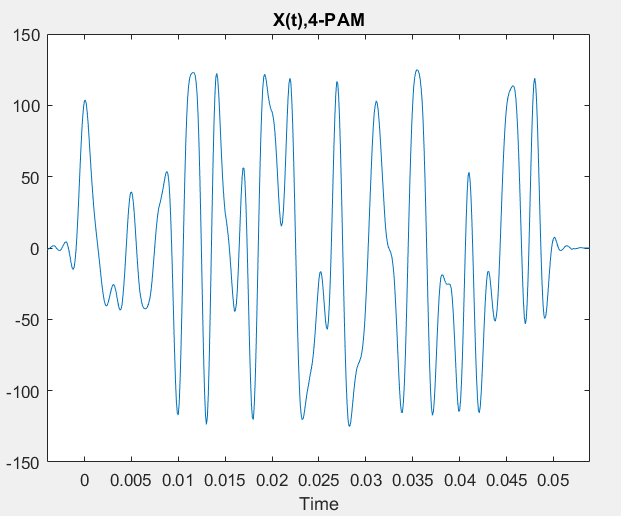
\includegraphics[width=0.8\textwidth]{ALPHA/images/a4.png} % Adjust width as neededfilename of your images
\end{center}


\begin{justify}
    (10) Να υπολογίσετε το περιοδόγραμμα και να εκτιμήσετε τη φασματική πυκνότητα
    ισχύος μέσω αριθμητικών μέσων τιμών υλοποιήσεων περιοδογραμμάτων της $X(\textlatin{t})$. Να
    σχεδιάσετε την πειραματική και την θεωρητική φασματική πυκνότητα ισχύος στο ίδιο
    \textlatin{semilogy}. Τι παρατηρείτε\textlatin{;}
\end{justify}

\begin{justify}
    {\bf Λύση:}\\\\
    Παρομοίως με το ερώτημα {\bf Α.3}, πραγματοποιήθηκε η εκτίμηση
    της φασματικής πυκνότητας ισχύος. Έπειτα, για να βρεθεί η 
    αντίστοιχη θεωρητική φασματική πυκνότητα ισχύος, ξαναχρησιμοποιήθηκε
    ο τύπος του {\bf Α.3}, με την διαφορά ότι η νέα
    διασπορά $\sigma_X^2$ είναι:
    \[
         \sigma_X^2 = E(X_n^2)=\sum x^2p_x=(1)^2\frac{1}{4}+(-1)^2\frac{1}{4}
         +(3)^2\frac{1}{4}+(-3)^2\frac{1}{4}=5
    \]
    Τέλος σχεδιάστηκαν και οι δύο σε ένα κοινό διάγραμμα με
    λογαριθμική κλίμακα.
\end{justify}

%%%%%%PLOT
\begin{center}
    \centering
    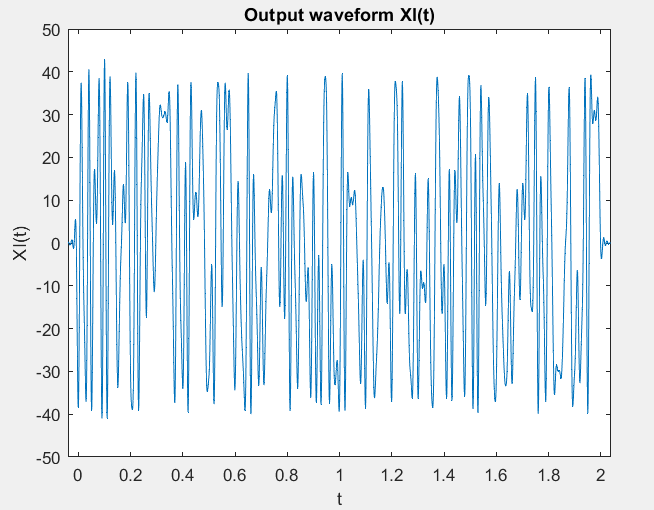
\includegraphics[width=0.8\textwidth]{ALPHA/images/a4.1.png} % Adjust width as neededfilename of your images
\end{center}



\begin{justify}
    Παρατηρούμε όμοια συμπεριφορά με το ερώτημα {\bf Α.3}, για το πλήθος
    των περιοδογραμμάτων Κ=500 που χρησιμοποιήθηκαν για την εκτίμηση.
\end{justify}

\begin{justify}
    και ο κώδικας \textlatin{Matlab}:
\end{justify}

\vspace{-0.8cm}

%%%%%%%%MATLAB code
\textlatin{
    \lstinputlisting[language=Matlab,]{ALPHA/Matlab/a4.1.m}
}



\begin{justify}
    (10) Πώς συγκρίνεται, ως προς το εύρος φάσματος και ως προς το μέγιστο πλάτος τιμών,
    η φασματική πυκνότητα ισχύος της $X(\textlatin{t})$ σε σχέση με αυτή της $X(\textlatin{t})$ του βήματος {\bf A.2}\textlatin{;}
    Μπορείτε να εξηγήσετε τα αποτελέσματα της σύγκρισης\textlatin{;}
\end{justify}

%%%%%%PLOT
\begin{center}
    \centering
    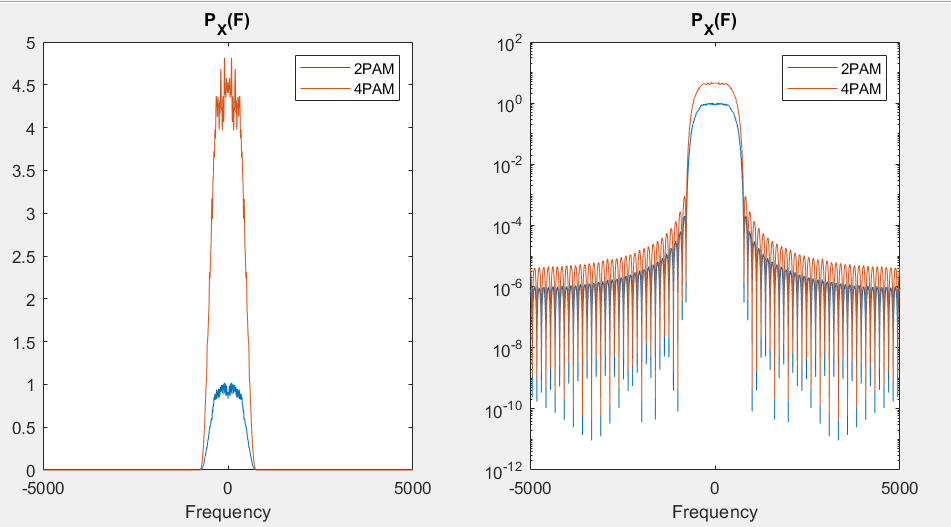
\includegraphics[width=0.8\textwidth]{ALPHA/images/a4.2.png} % Adjust width as neededfilename of your images
\end{center}


\begin{justify}
    {\bf Λύση:}\\\\
    Απεικονίσαμε σε κοινό \textlatin{plot} και \textlatin{semilogy}
    τις φασματικές πυκνότητες ισχύος 2-\textlatin{PAM} και
    4-\textlatin{PAM}. Παρατηρούμε ότι το εύρος φάσματος και των δύο
    είναι ίδιο αφού $BW=\frac{1+\alpha}{2Τ}$, το οποίο εξαρτάται μόνο
    από την συχνότητα $T$ και το $\alpha$. Στην συνέχεια, Παρατηρούμε
    ότι το μέγιστο πλάτος των τιμών της 4-\textlatin{PAM} είναι σχεδόν
    5 φορές μεγαλύτερο έναντι με αυτού της 2-\textlatin{PAM} και αυτό
    συμβαίνει διότι η διασπορά της 4-\textlatin{PAM} είναι μεγαλύτερη.
\end{justify}

\begin{justify}
    και ο κώδικας \textlatin{Matlab}:
\end{justify}

\vspace{-0.8cm}

%%%%%%%%MATLAB code
\textlatin{
    \lstinputlisting[language=Matlab,]{ALPHA/Matlab/a4.2.m}
}

\newpage

%%%%%%%%%%%%%%%%%  A5

\begin{justify}
    {\bf A.5} (10) Να επαναλάβετε το βήμα Α.3, θέτοντας περίοδο συμβόλου $T' = 2T$ (να διατηρήσετε
    την περίοδο δειγματοληψίας $T_s$ ίση με αυτή των προηγούμενων βημάτων, άρα, θα πρέπει
    να διπλασιάσετε την παράμετρο \textlatin{over}).
\end{justify}

\begin{justify}
    {\bf Λύση:}\\\\
    Ακολουθήθηκε η ίδια διαδικασία με το ερώτημα {\bf Α.3}, 
    με $Τ'=2\cdot10^-3$ και $over'=20$. Παρακάτω παρουσιάζεται το 
    περιοδόγραμμα $P_X(F)$ σε δεκαδική και λογαριθμική κλίμακα:
\end{justify}

%%%%%%PLOT
\begin{center}
    \centering
    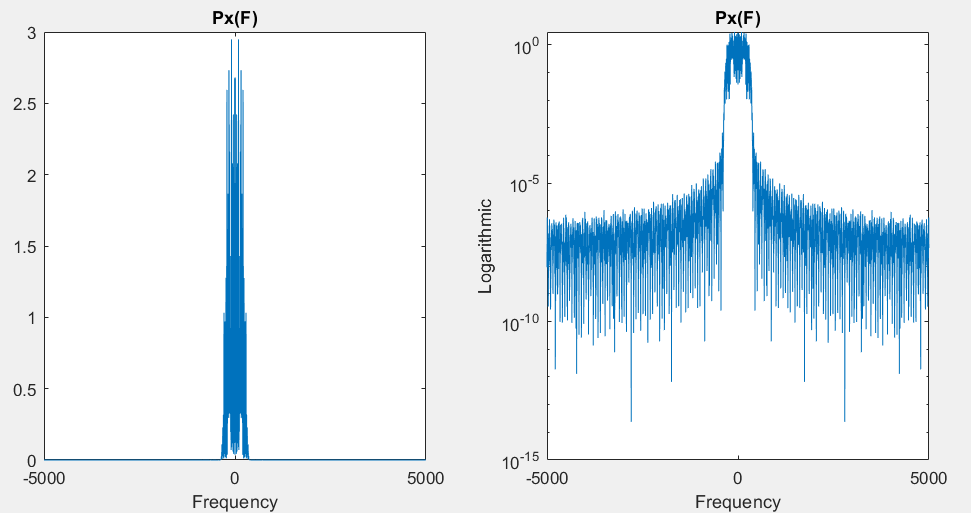
\includegraphics[width=0.8\textwidth]{ALPHA/images/a5.1.png} % Adjust width as neededfilename of your images
\end{center}

\vspace{-0.8cm}

%%%%%%%%MATLAB code
\textlatin{
    \lstinputlisting[language=Matlab,]{ALPHA/Matlab/a5.1.m}
}


\begin{justify}
    Και  όμοια πάλι με το ερώτημα
    {\bf Α.3}, προκύπτει το κοινό διάγραμμα για την θεωρητική και την 
    εκτιμόμενη φασματική πυκνότητα ισχύος:
\end{justify}


%%%%%%PLOT
\begin{center}
    \centering
    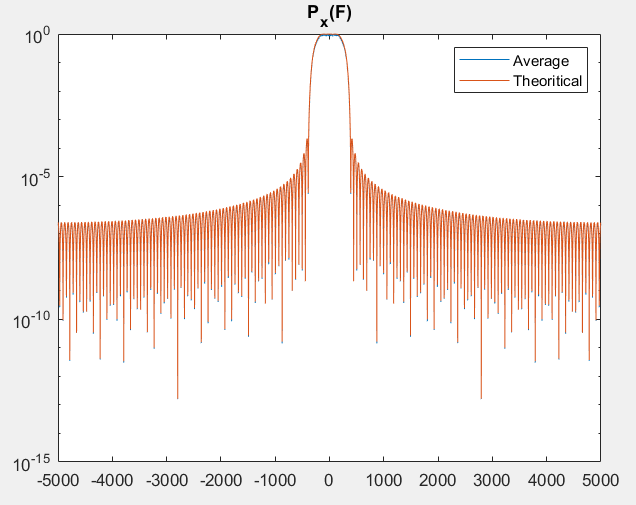
\includegraphics[width=0.6\textwidth]{ALPHA/images/a5.2.png} % Adjust width as neededfilename of your images
\end{center}

\vspace{-0.8cm}

%%%%%%%%MATLAB code
\textlatin{
    \lstinputlisting[language=Matlab,]{ALPHA/Matlab/a5.2.m}
}

\newpage

\begin{justify}
    Τέλος χρησιμοποιώντας διαφορετικά Κ και Ν προκύπτουν τα παρακάτω
    διαγράμματα:
\end{justify}

%%%%%%PLOT
\begin{center}
    \centering
    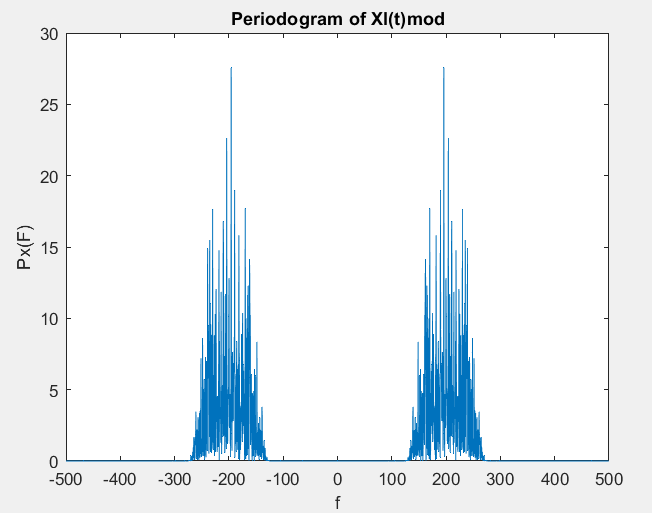
\includegraphics[width=0.8\textwidth]{ALPHA/images/a5.3.png} % Adjust width as neededfilename of your images
\end{center}

\begin{justify}
    (5) Τι παρατηρείτε σχετικά με το εύρος φάσματος 
    των κυματομορφών σε αυτή την
    περίπτωση σε σχέση με αυτό των κυματομορφών 
    του βήματος Α.3\textlatin{;} Μπορείτε να εξηγήσετε το φαινόμενο\textlatin{;}
\end{justify}

\begin{justify}
    {\bf Λύση:}\\\\
    Κάνοντας κοινό \textlatin{plot} των περιοδογραμμάτων των 2
    ερωτημάτων:
\end{justify}

%%%%%%PLOT
\begin{center}
    \centering
    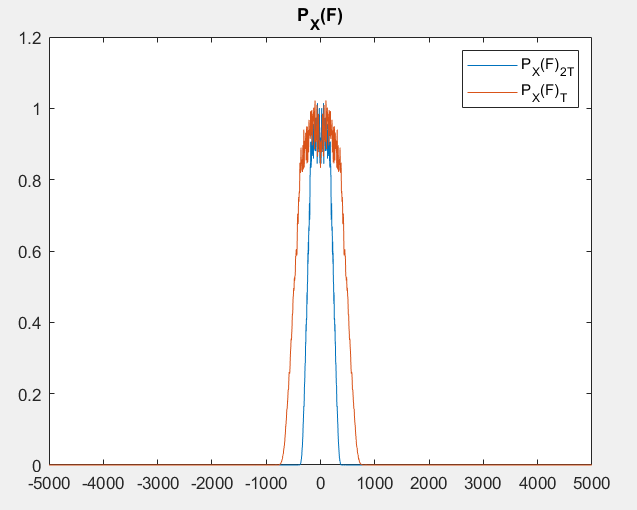
\includegraphics[width=0.6\textwidth]{ALPHA/images/a5.4.png} % Adjust width as neededfilename of your images
\end{center}



\begin{justify}
    Γίνεται εύκολα αντιληπτό ότι για $T'=2T$ μείωνεται εμφανώς το
    το εύρος φάσματος, πράγμα που επιβεβαιώνεται και από την θεωρία αφού
    $BW=\frac{1+\alpha}{2Τ}$.
\end{justify}

\newpage

%%%%%%%%%%%%%%%%%%%%%%%%%%%%%%  A6

\begin{justify}
    {\bf Α.6} (2.5) Αν θέλατε να στείλετε δεδομένα
    όσο το δυνατό ταχύτερα έχοντας διαθέσιμο το ίδιο εύρος
    φάσματος, θα επιλέγατε \textlatin{2-PAM} ή \textlatin{4-PAM},
    και γιατί\textlatin{;}    
\end{justify}

\begin{justify}
    {\bf Λύση:}\\\\
    Για να επιτευχθεί η ταχύτερη διάδοση δεδομένων έχοντας διαθέσιμο
    το ίδιο εύρος φάσματος, θα επιλέγαμε \textlatin{4-PAM} καθώς 
    αντιστοιχίζονται δύο \textlatin{bits} ανα σύμβολο σε αντίθεση
    με το \textlatin{2-PAM} που αντιστοιχίζεται ένα. Επομένως στέλνονται
    περισσότερα \textlatin{bits} πληροφορίας στον ίδιο χρόνο.
\end{justify}

\begin{justify}
    (2.5) Αν το διαθέσιμο εύρος φάσματος είναι πολύ ακριβό,
    θα επιλέγατε περίοδο συμβόλου $Τ$ ή $Τ'=2T$, και γιατί\textlatin{;}
\end{justify}

\begin{justify}
    {\bf Λύση:}\\\\
    Αν το διαθέσιμο εύρος φάσματος είναι πολύ ακριβό, θα επιλέγαμε
    περίοδο συμβόλου $Τ'=2T$ καθώς, όπως δείξαμε και στο ερώτημα
    {\bf Α.5}, θα έδινε μικρότερο εύρος φάσματος και έτσι θα εξοικονομούνταν
    στην μετάδοση το μισό φάσμα.
\end{justify}



\newpage

\begin{justify}
    {\bf  Β.1}\\
    Για $T=10^{-2}$, $A=4$, $a=0,0.5,1$ και $k=0,1...,2A$(αντίστοιχα
    αποτελέσματα θα πάρετε για αρνητικά $k$)\\
    1.να σχεδιάσετε σε κοινό \textlatin{plot} τους παλμούς $\phi(t)$ 
    και $\phi(t-kT)$,\\
    2.να σχεδιάσετε το γινόμενο $\phi(t)\phi(t-kT)$,\\
    3.να προσεγγίσετε αριθμητικά το ολοκλήρωμα του
    γινομένου $\phi(t)\phi(t-kT)$, με τη μέθοδο που αναφέρουμε
    στις σημειώσεις.\\

    {\bf (α)} (10) Να σχεδιάσετε τα αποτελέσματα των βημάτων
    1. και 2. για $a=0,0.5,1$ και $k=0,1,2$:\\\\
    \textbf{Λύση:}\\
\end{justify}

\begin{justify}
    Οι παλμοί $\phi(t)$ και $\phi(t-kT)$:
\end{justify}

%%%%%%PLOT
\begin{center}
    \centering
    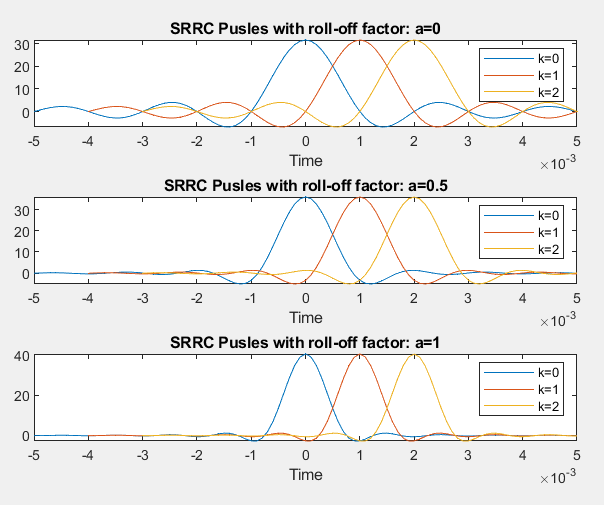
\includegraphics[width=0.8\textwidth]{BETA/Images/B1.1.png} % Adjust width as neededfilename of your images
\end{center}

\newpage

\begin{justify}
Καθώς και το γινόμενο $\phi(t)\phi(t-kT)$:     
\end{justify}


%%%%%%PLOT
\begin{center}
    \centering
    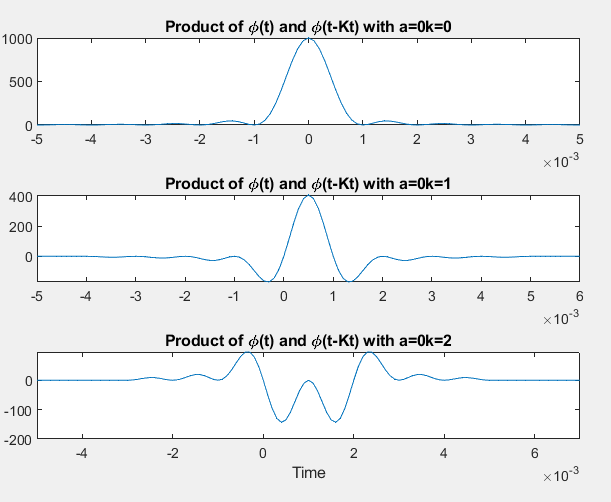
\includegraphics[width=0.8\textwidth]{BETA/Images/B2.1.png} % Adjust width as neededfilename of your images
\end{center}


%%%%%%PLOT
\begin{center}
    \centering
    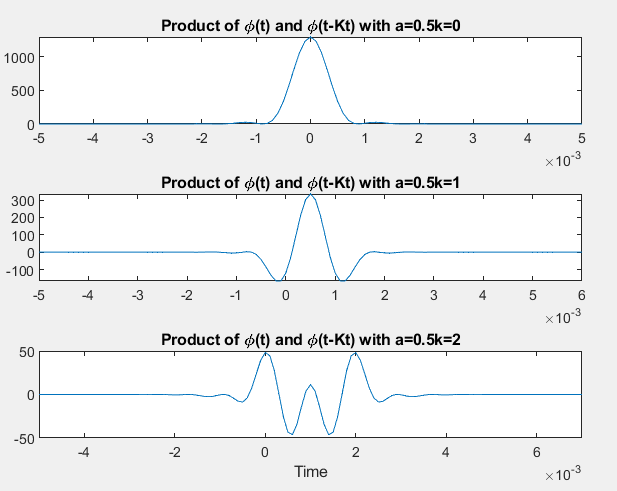
\includegraphics[width=0.8\textwidth]{BETA/Images/B2.2.png} % Adjust width as neededfilename of your images
\end{center}


%%%%%%PLOT
\begin{center}
    \centering
    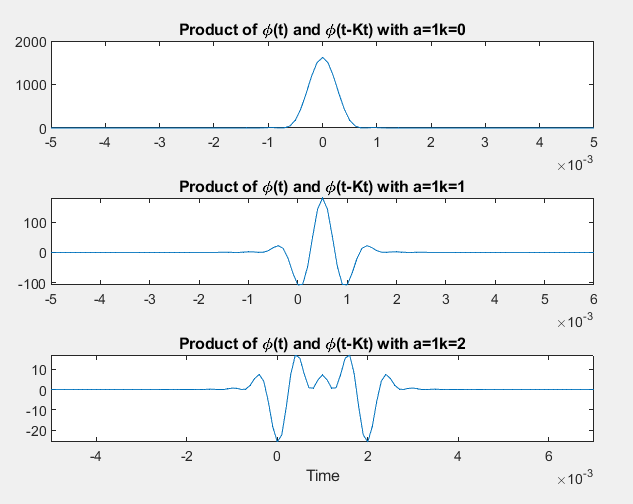
\includegraphics[width=0.8\textwidth]{BETA/Images/B2.3.png} % Adjust width as neededfilename of your images
\end{center}





\begin{justify}
    {\bf (β)} (10) Να αναφέρετε τις τιμές των ολοκληρωμάτων
    που υπολογίσατε στο βήμα 3., για $a=0,0.5,1$ και $k=0,1,2,3$
    και να προσπαθήσετε να τις εξηγήσετε.\\\\
    \textbf{Λύση:}\\
    Για $α=0$:\\
        $\int_{-\infty}^{+\infty}\phi(t)\phi(t-0T)\,dt=0.974749$\\
        $\int_{-\infty}^{+\infty}\phi(t)\phi(t-1T)\,dt=0.029027$\\
        $\int_{-\infty}^{+\infty}\phi(t)\phi(t-2T)\,dt=-0.034885$\\
        $\int_{-\infty}^{+\infty}\phi(t)\phi(t-3T)\,dt=0.046111$\\
\end{justify}    

\begin{justify}
Για $α=0.5$:\\
    $\int_{-\infty}^{+\infty}\phi(t)\phi(t-0T)\,dt=0.999876$\\
    $\int_{-\infty}^{+\infty}\phi(t)\phi(t-1T)\,dt=0.000022$\\
    $\int_{-\infty}^{+\infty}\phi(t)\phi(t-2T)\,dt=0.000333$\\
    $\int_{-\infty}^{+\infty}\phi(t)\phi(t-3T)\,dt=-0.000341$\\\\
\end{justify}

\newpage

\begin{justify}
Για $α=1$:\\
    $\int_{-\infty}^{+\infty}\phi(t)\phi(t-0T)\,dt=0.999969$\\
    $\int_{-\infty}^{+\infty}\phi(t)\phi(t-1T)\,dt=-0.000047$\\
    $\int_{-\infty}^{+\infty}\phi(t)\phi(t-2T)\,dt=-0.000082$\\
    $\int_{-\infty}^{+\infty}\phi(t)\phi(t-3T)\,dt=-0.000203$  
\end{justify}

\begin{justify}
    Παρατηρούμε ότι για όλες τις διαφορετικές τιμές του $a$
    για $k=0$ οι τιμές των ολοκληρωμάτων προσεγγίζουν το 1.
    Αντιθέτως για $k\neq0$ έχουμε τιμές που προσεγγίζουν το 0.
    Άρα συμπεραίνουμε ότι οι παλμοί που δημιουργήσαμε είναι κατα
    προσσέγιση ορθοκανονικοί.\\\\
    Ακολουθεί ο κώδικας \textlatin{Matlab} για τα παραπάνω ερωτήματα:
\end{justify}

\vspace{-1cm}

%%%%%%%%MATLAB code
\textlatin{
    \lstinputlisting[language=Matlab,]{BETA/Matlab/B1.m}
}
       




\newpage

\begin{justify}
    Στο 3\textsuperscript{ο} και τελευταίο ερώτημα, θα προσομοιωθεί
    ένα \textlatin{PAM} σύστμα βασικής ζώνης, το οποίο μεταφέρει
    $N$ \textlatin{bits} χρησιμοποιώντας διαμόρφωση \textlatin{2-PAM}.
    Για $T=10^{-2}$\textlatin{sec}, \textlatin{over}$=10$, $α=0.5$,
    και $Α=4$. (το $Α$ ισούται με το μισό μήκος του αποκομμένου 
    παλμού μετρημένο σε περιόδους συμβόλου).\\\\
    {\bf \textlatin{C.1}} (5) Να δημιοργήσετε $N$ \textlatin{bits}
    $b\textsubscript{i}$ για $i=0,1,..N-1$ ($N=50,100$), με την
    εντολή $b=(sign(rand(N,1))+1)/2$:\\\\
    \textbf{Λύση:}
\end{justify}

\vspace{-2em}
    
%%%%%%%%MATLAB code
\textlatin{
    \lstinputlisting[language=Matlab,]{CE/Matlab/C1.m}
} 

\begin{justify}
    {\bf \textlatin{C.2}} Το σύστημα \textlatin{2-PAM} υλοποιείται
    ως εξής.\\\\
    {\bf (α)} (5) Να γράψετε την συνάρτηση
    $X=bits\_to\_2PAM(b)$ η οποία παίρνει είσοδο την ακολουθία
    \textlatin{bits b} και παράγει ως έξοδο την ακολουθία από
    \textlatin{2-PAM} σύμβολα $X$, χρησιμοποιώντας την εξής απεικόνιση:
    \[ 0 \rightarrow +1, \]
    \[ 1 \rightarrow -1. \]
\end{justify}

\begin{justify}
    \textbf{Λύση:}\\
    Η συνάρτηση επιστρέφει $X=-1$ με είσοδο $b=1$ και 
    $X=1$ όταν $b=0$.

\end{justify}

\vspace{-2em}

%%%%%%%%MATLAB code
\textlatin{
    \lstinputlisting[language=Matlab,]{CE/Matlab/C2A.m}
} 

\newpage

\begin{justify}
    {\bf (β)} Να προσομοιώσετε το σήμα:
\end{justify}

\[
    X_{\delta}(t)=\sum_{k=0}^{N-1}X_{k}\delta(t-kT)
\]

\begin{justify}
μέσω της εντολής:
\end{justify}
\[
    X\_delta=1/Ts*upsample(X,over).
\]

\begin{justify}
    (10) Να ορίσετε κατάλληλα τον άξονα του χρόνου και να σχεδιάσετε
    το σήμα $X_{\delta}(t)$.\\\\
    \textbf{Λύση:}
\end{justify}
    
\vspace{-2em}

%%%%%%%%MATLAB code
\textlatin{
    \lstinputlisting[language=Matlab,]{CE/Matlab/C2B.m}
} 

\newpage

\begin{justify}
    Όπως βλέπουμε σχεδιάσαμε ένα τρένο παλμών κλιμακομένο κατά 
    $1/T_{s}$.
\end{justify}

%%%%%%PLOT
\begin{center}
    \centering
    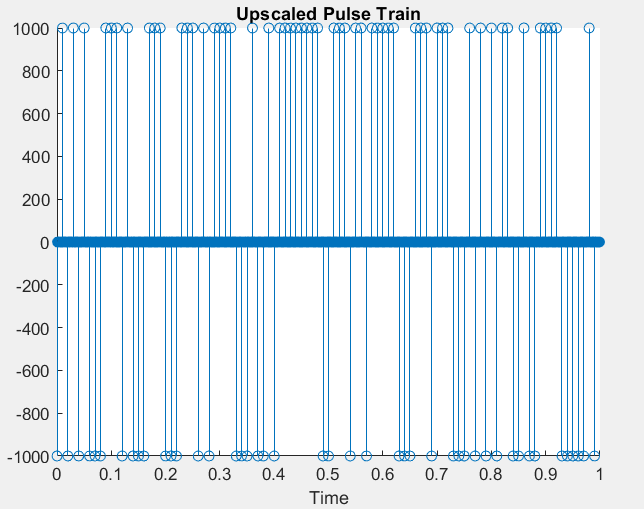
\includegraphics[width=0.8\textwidth]{CE/Images/c.1.png} % Adjust width as neededfilename of your images
\end{center}



\begin{justify} 
    {\bf (ς)} Να δημιουργήσετε αποκομμένο \textlatin{SRRC}
    παλμός $\phi(t)$(χρησιμοποιώντας τις παραπάνω παραμέτρους) και 
    να προσομοιώσετε την συνέλιξη $X(t)=X_{\delta}*\phi(t)$.\\\\
    (10) Να κατασκευάσετε κατάλληλα τον άξονα
    του χρόνου και να σχεδιάσετε το σήμα $X(t)$.\\\\
\end{justify}

\vspace{-2em}

%%%%%%%%MATLAB code
\textlatin{
    \lstinputlisting[language=Matlab,]{CE/Matlab/C3.m}
} 

\newpage

%%%%%%PLOT
\begin{center}
    \centering
    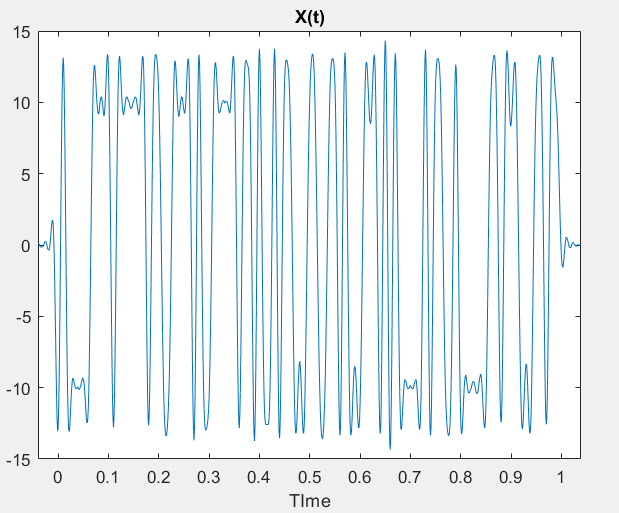
\includegraphics[width=0.8\textwidth]{CE/Images/c.2.png} % Adjust width as neededfilename of your images
\end{center}

\vspace{1.5em}

\begin{justify}
    {\bf (δ)} Υποθέτοντας ιδανικό κανάλι, στην είσοδο του δέκτη
    λαμβάνουμε $X(t)$. Να προσομοιώσετε τη συνέλιξη $Z(t)=X(t)*\phi(-t)$.\\\\
    (10) Να σχεδιάσετε το $Z(t)$ στον αντίστοιχο άξονα του χρόνου
    και να βρείτε τι τιμές παίρνει τις χρονικές στιγμές $kT$, για
    $k=0,...,N-1$.Μπορείτε να εξηγήσετε το φαινόμενο\textlatin{;}\\\\
    \textbf{Λύση:}\\
    Χρησιμοποιήθηκε ο ίδιος αποκομμένος \textlatin{SRRC} παλμός
    διότι είναι άρτια συνάρτηση ($\phi(t)=\phi(-t)$).
\end{justify}

\vspace{-2em}

%%%%%%%%MATLAB code
\textlatin{
    \lstinputlisting[language=Matlab,]{CE/Matlab/C4.1.m}
} 

%%%%%%PLOT
\begin{center}
    \centering
    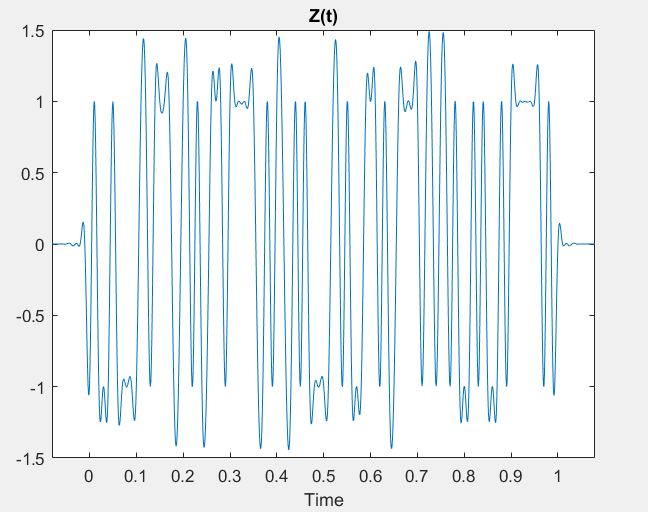
\includegraphics[width=0.8\textwidth]{CE/Images/c.3.png} % Adjust width as neededfilename of your images
\end{center}

\begin{justify}
    (5) Ένας γραφικός τρόπος για να συγκρίνεται τις τιμές
    $Z(kT)$ με τις τιμές $X_{k}$, για  $k=0,...,N-1$, είναι να
    επιλέξετε \textlatin{hold on} στο \textlatin{plot} του
    $Z(t)$ και να εκτελέσετε την εντολή \textlatin{stem([0:N-1]*T,X);}
    όπου $Χ$ είναι το διάνυσμα με τα σύμβολα $X_{k}$, $k=0,...,N-1$.\\\\
    \textbf{Λύση:}\\
\end{justify}

\begin{justify}
    Βρίσκουμε τις θέσεις του $Z(t)$ που μας ενδοιαφέρουν
    δηλαδή από την χρονική στιγμή $t=0$ ως την χρομνική στιγμή
    που τελειώνει το τρένο παλμών. Έχοντας τον παλμό που μας ενδοιαφέρει
    \textlatin{zsampled} τον κάνουμε \textlatin{downsample}.\\\\
    Ακολουθεί ο κώδικας \textlatin{Matlab}: 
\end{justify}

\vspace{-2em}

%%%%%%%%MATLAB code
\textlatin{
    \lstinputlisting[language=Matlab,]{CE/Matlab/C4.2.m}
} 

%%%%%%PLOT
\begin{center}
    \centering
    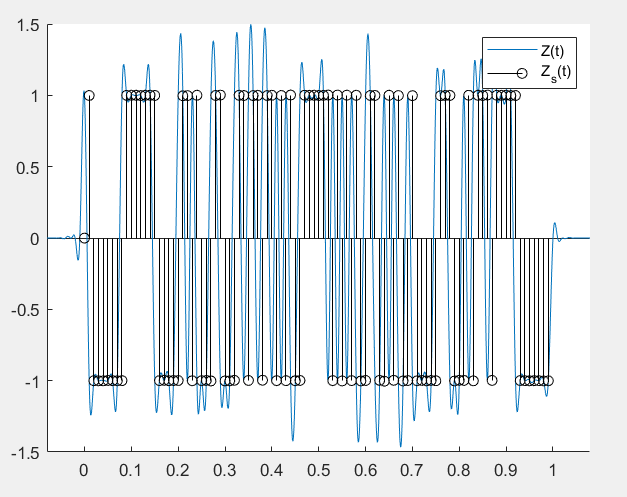
\includegraphics[width=0.8\textwidth]{CE/Images/c.4.png} % Adjust width as neededfilename of your images
\end{center}







\end{document}